\documentclass[tikz,border=6pt]{standalone}
\usepackage{amsmath}
\usepackage{amssymb}
\usetikzlibrary{arrows.meta,positioning,calc,fit,backgrounds}

\begin{document}
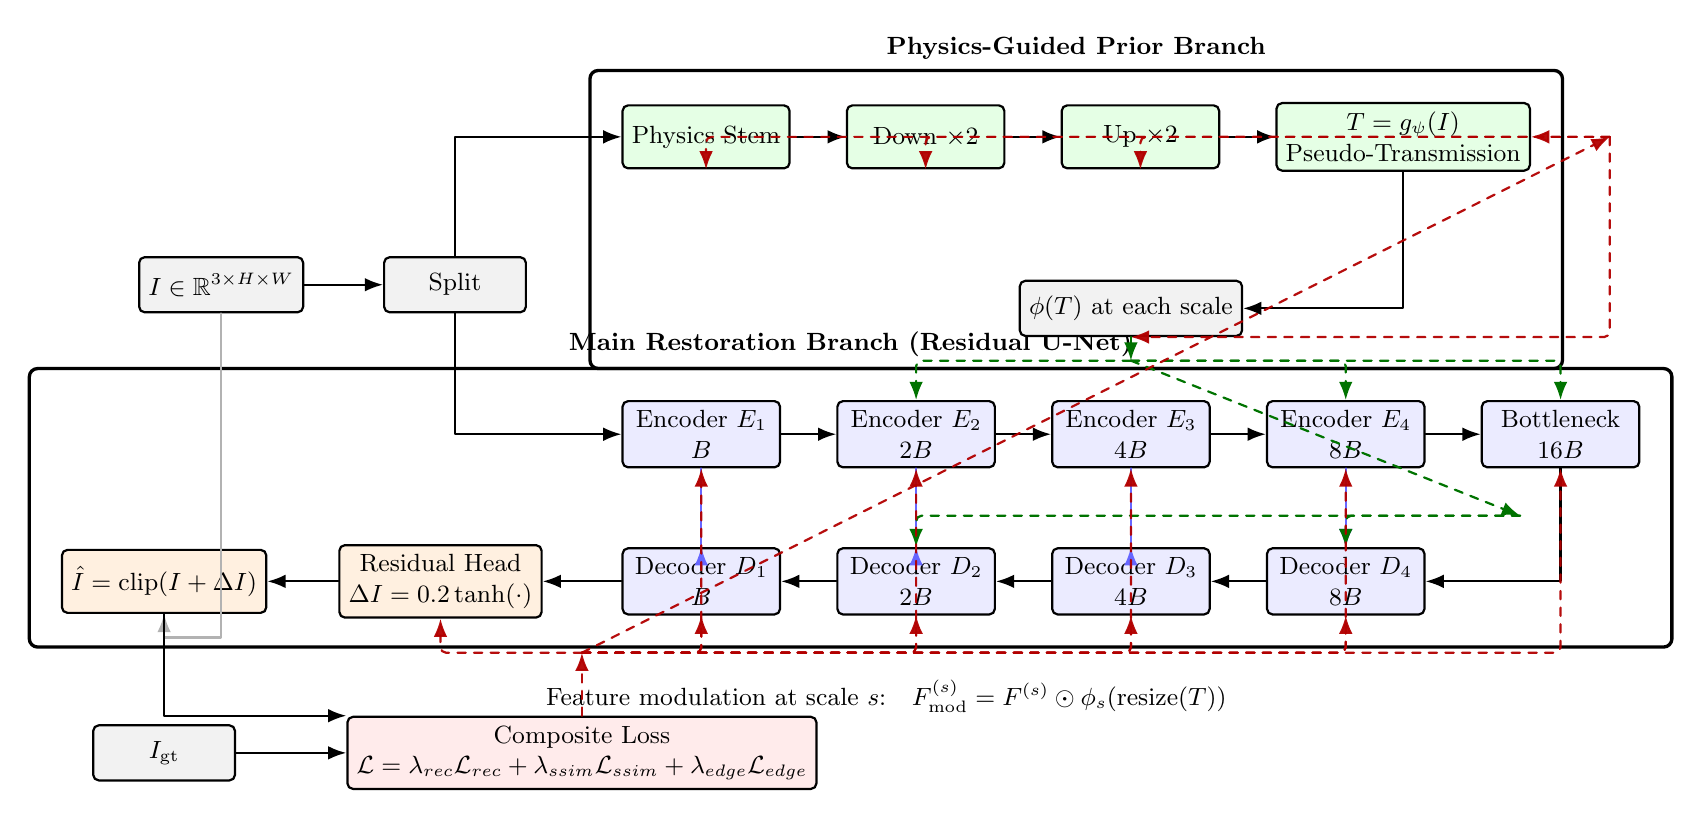
\begin{tikzpicture}[
    font=\small,
    >=Latex,
    line cap=round,
    line join=round,
    block/.style={draw, rounded corners=2pt, thick, align=center, minimum width=20mm, minimum height=8mm},
    op/.style={draw, rounded corners=2pt, thick, align=center, minimum width=18mm, minimum height=7mm, fill=gray!10},
    enc/.style={block, fill=blue!8},
    dec/.style={block, fill=blue!8},
    prior/.style={block, fill=green!10},
    outblk/.style={block, fill=orange!12},
    trainblk/.style={block, fill=red!8},
    flow/.style={->, thick},
    skip/.style={->, thick, blue!60},
    mod/.style={->, thick, dashed, green!45!black, rounded corners=2pt},
    bp/.style={->, thick, dashed, red!70!black, rounded corners=2pt, opacity=0.95}
]

% ------------------------
% Inputs and split
% ------------------------
\node[op] (input) {$I \in \mathbb{R}^{3\times H\times W}$};
\node[op, right=10mm of input] (split) {Split};
\draw[flow] (input.east) -- (split.west);

% ------------------------
% Physics-guided prior branch
% ------------------------
\node[prior, above right=11mm and 12mm of split] (pstem) {Physics Stem};
\node[prior, right=7mm of pstem] (pdown) {Down $\times 2$};
\node[prior, right=7mm of pdown] (pup) {Up $\times 2$};
\node[prior, right=7mm of pup] (tmap) {$T=g_{\psi}(I)$\\Pseudo-Transmission};

\draw[flow] (split.north) |- (pstem.west);
\draw[flow] (pstem.east) -- (pdown.west);
\draw[flow] (pdown.east) -- (pup.west);
\draw[flow] (pup.east) -- (tmap.west);

% ------------------------
% Main restoration branch (Residual U-Net)
% ------------------------
\node[enc, below right=11mm and 12mm of split] (e1) {Encoder $E_1$\\$B$};
\node[enc, right=7mm of e1] (e2) {Encoder $E_2$\\$2B$};
\node[enc, right=7mm of e2] (e3) {Encoder $E_3$\\$4B$};
\node[enc, right=7mm of e3] (e4) {Encoder $E_4$\\$8B$};
\node[enc, right=7mm of e4] (bott) {Bottleneck\\$16B$};

\node[dec, below=10mm of e4] (d4) {Decoder $D_4$\\$8B$};
\node[dec, left=7mm of d4] (d3) {Decoder $D_3$\\$4B$};
\node[dec, left=7mm of d3] (d2) {Decoder $D_2$\\$2B$};
\node[dec, left=7mm of d2] (d1) {Decoder $D_1$\\$B$};

\node[outblk, left=10mm of d1] (head) {Residual Head\\$\Delta I=0.2\tanh(\cdot)$};
\node[outblk, left=9mm of head] (sum) {$\hat I=\mathrm{clip}(I+\Delta I)$};

\draw[flow] (split.south) |- (e1.west);
\draw[flow] (e1.east) -- (e2.west);
\draw[flow] (e2.east) -- (e3.west);
\draw[flow] (e3.east) -- (e4.west);
\draw[flow] (e4.east) -- (bott.west);

\draw[flow] (bott.south) |- (d4.east);
\draw[flow] (d4.west) -- (d3.east);
\draw[flow] (d3.west) -- (d2.east);
\draw[flow] (d2.west) -- (d1.east);
\draw[flow] (d1.west) -- (head.east);
\draw[flow] (head.west) -- (sum.east);

% Input-to-output residual add context (optional visual hint)
\draw[flow, gray!60] (input.south) |- ([yshift=-3mm]sum.south) -- (sum.south);

% ------------------------
% U-Net skip links (explicit orthogonal routing)
% ------------------------
\draw[skip] (e4.south) -- ++(0,-3mm) -- (d4.north);
\draw[skip] (e3.south) |- (d3.north);
\draw[skip] (e2.south) |- (d2.north);
\draw[skip] (e1.south) |- (d1.north);

% ------------------------
% Modulation stream
% ------------------------
\node[op, above=8mm of e3] (phi) {$\phi(T)$ at each scale};
\draw[flow] (tmap.south) |- (phi.east);

% Fan-out bus to avoid overlapping dashed arrows
\coordinate (mbusTop) at ($(phi.south)+(0,-3mm)$);
\coordinate (mbusDec) at ($(d4.north east)+(12mm,4mm)$);
\draw[mod] (phi.south) -- (mbusTop);
\draw[mod] (mbusTop) -- (mbusDec);

% Encoder/Bottleneck modulation taps
\draw[mod] (mbusTop) -| (e2.north);
\draw[mod] (mbusTop) -| (e4.north);
\draw[mod] (mbusTop) -| (bott.north);

% Decoder modulation taps (routed from dedicated decoder lane)
\draw[mod] (mbusDec) -| (d4.north);
\draw[mod] (mbusDec) -| (d2.north);

% ------------------------
% Equation
% ------------------------
\node[align=left, below=7mm of d2, text width=9.4cm] (eq)
{Feature modulation at scale $s$:\quad
$F^{(s)}_{\mathrm{mod}} = F^{(s)} \odot \phi_s\!\left(\mathrm{resize}(T)\right)$};

% ------------------------
% Training loss + backprop flow
% ------------------------
\node[op, below=14mm of sum] (gt) {$I_{\mathrm{gt}}$};
\node[trainblk, right=14mm of gt, minimum width=30mm] (loss)
{Composite Loss\\$\mathcal{L}=\lambda_{rec}\mathcal{L}_{rec}+\lambda_{ssim}\mathcal{L}_{ssim}+\lambda_{edge}\mathcal{L}_{edge}$};

\draw[flow] (sum.south) |- (loss.north west);
\draw[flow] (gt.east) -- (loss.west);

% Full gradient paths (backpropagation) to all trainable modules
\coordinate (bpbus) at ($(loss.north)+(0,8mm)$);
\coordinate (bpprior) at ($(tmap.east)+(10mm,0)$);
\draw[bp] (loss.north) -- (bpbus);

% Main branch
\draw[bp] (bpbus) -| (head.south);
\draw[bp] (bpbus) -| (d1.south);
\draw[bp] (bpbus) -| (d2.south);
\draw[bp] (bpbus) -| (d3.south);
\draw[bp] (bpbus) -| (d4.south);
\draw[bp] (bpbus) -| (bott.south);
\draw[bp] (bpbus) -| (e4.south);
\draw[bp] (bpbus) -| (e3.south);
\draw[bp] (bpbus) -| (e2.south);
\draw[bp] (bpbus) -| (e1.south);

% Modulation + physics prior branch
\draw[bp] (bpbus) -- (bpprior);
\draw[bp] (bpprior) |- (phi.south);
\draw[bp] (bpprior) -- (tmap.east);
\draw[bp] (bpprior) -| (pup.south);
\draw[bp] (bpprior) -| (pdown.south);
\draw[bp] (bpprior) -| (pstem.south);

% ------------------------
% Branch grouping boxes
% ------------------------
\begin{scope}[on background layer]
    \node[draw, rounded corners=3pt, very thick, inner sep=4mm,
          fit=(pstem)(pdown)(pup)(tmap)(phi),
          label=above:{\textbf{Physics-Guided Prior Branch}}] {};
    \node[draw, rounded corners=3pt, very thick, inner sep=4mm,
          fit=(e1)(bott)(d1)(sum),
          label=above:{\textbf{Main Restoration Branch (Residual U-Net)}}] {};
\end{scope}

\end{tikzpicture}
\end{document}
